\documentclass[11pt]{article}
\usepackage[margin=1in]{geometry}
\usepackage[T1]{fontenc}
\usepackage{lmodern}
\input{ot1lmr.fd}
\DeclareFontShape{T1}{lmr}{m}{n}{<-> ec-lmr10}{}
\DeclareFontShape{T1}{lmr}{m}{it}{<-> ec-lmri10}{}
\DeclareFontShape{OT1}{lmr}{m}{n}{<-> rm-lmr10}{}
\input{omllmm.fd}
\DeclareFontShape{OML}{lmm}{m}{it}{<-8.5> lmmi8 <8.5-> lmmi10}{}
\input{omslmsy.fd}
\DeclareFontShape{OMS}{lmsy}{m}{n}{<-8.5> lmsy8 <8.5-> lmsy10}{}
\usepackage{amsmath,amssymb,booktabs,graphicx,microtype}
\usepackage[hidelinks]{hyperref}
\urlstyle{same}
\setlength{\emergencystretch}{2em}
\clubpenalty=10000\widowpenalty=10000
\title{Shaping Gap Benchmark V:\\Learned Component Execution\\Beyond the Transformer Graph}
\author{Nathaniel Oh \and Paul Attie}
\date{November 13, 2026}
\begin{document}
\maketitle
\begin{abstract}
Can the learning and compatibility cycle of a neural runtime operate directly over pretrained components, after replacing the original transformer execution graph? We extract fixed neural fragments from two pretrained language-model sizes, acquire response interfaces from native values and partial derivatives, and use their accumulated interaction effects to route component execution. A response-derived recurrent return change and a shared observation map form an acquired executable pair. Experiential feedback selects a pair before untouched input streams validate reuse. Across six pretrained component contexts, one pair improves nonlinear temporal-processing quality on both fresh streams while retaining its two eligible old programs; five contexts retain baseline. Mean quality changes over all six are positive and all 18 old program instances remain usable. First-order guidance yields two strict successes, and shuffled-conditioning and norm-matched random-weight controls each yield one. Independent replay reproduces 1,440 score vectors and checks 4,800 component-field outputs in original activation coordinates. The experiment executes no transformer blocks, attention, tokenizer or language-generation head. It establishes one finite acquisition and compatible-reuse cycle in a component runtime, with construction grammar, numerical fidelity, preparation costs and full controls explicit.
\end{abstract}

\section{From a pretrained body to an acquired component runtime}
A pretrained model supplies numerical components as well as a conventional way to connect them. This study asks whether useful computation and an experiential improvement cycle can operate after replacing that conventional graph. The source models provide frozen feed-forward components; the runtime acquires response interfaces, constructs a recurrent computation, and selects an execution change together with a shared interface for its old programs.

Checkpoint IV demonstrated experience-acquired execution and compatibility reuse around a complete frozen transformer body~\cite{sg4}. Checkpoints I and II supplied component-level effect interfaces and composition experiments~\cite{sg1,sg2}. Here the two lines meet: the acquisition, selection, retention and fresh-validation cycle operates directly on parameter-backed components. Original layer order and attention are absent from the deployed computation.

The measured contribution is this executable component cycle. Native-response interfaces guide the interaction of fragments, native geometry supplies return changes, paired trajectories supply compatibility, and feedback determines the pair retained for new inputs. The benchmark measures numerical temporal computation; it supplies no language question-answering outcome.

\begin{figure}[ht]\centering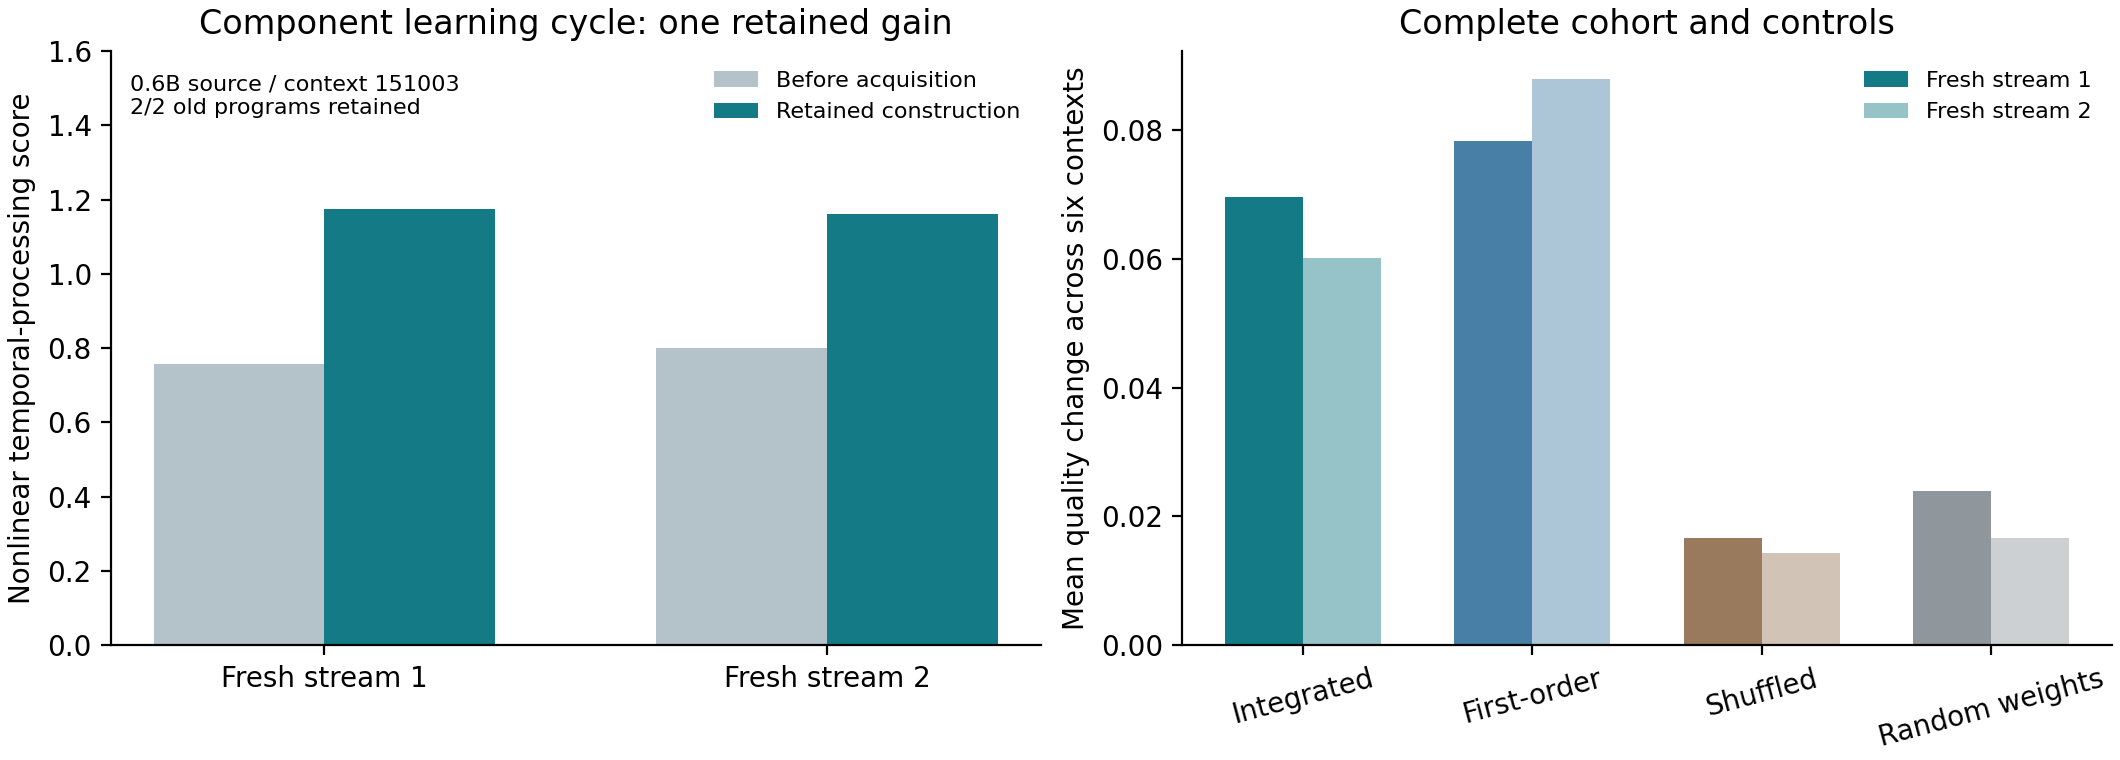
\includegraphics[width=\linewidth]{checkpoint-overview.png}
\caption{Left: the one strict integrated-guidance success, with two old programs retained. Right: mean changes across all six contexts for each guidance/control variant; baseline fallbacks are included. First-order guidance has larger mean improvement in this study.}\label{fig:overview}
\end{figure}

\section{Frozen fragments and the replacement execution graph}
\subsection{Physical inventory and numerical fidelity}
For each of three declared seeds in each of the pinned Qwen3-0.6B and Qwen3-1.7B four-bit checkpoints, we uniformly sample 24 physical SwiGLU units across the 28 original layers. Hidden widths are 1,024 and 2,048. No producer is chosen using task outcomes. The primitive at unit $i$ retains its gate row $g_i$, up row $u_i$, native normalization $N_i$ and down-projection column $d_i$:
\begin{equation}
 a_i(x)=\operatorname{SiLU}(g_i^\top N_i(x))\,u_i^\top N_i(x),\qquad f_i(x)=d_i a_i(x).
\end{equation}
The native normalization scale is absorbed into the materialized input rows. These arrays remain fixed. A norm-matched Gaussian control replaces gate, up and down rows while preserving their dimensions and row norms; it retains the same input anchor construction and numerical grammar.

Extraction uses the original frozen modules under guards against whole-model, transformer-body, transformer-block, attention, embedding and language-head calls. Three probes per bank compare materialized amplitudes and selected writes with the original mixed-precision modules. The maximum relative discrepancy across these checks is 0.01909. Thus extraction is a numerical materialization, not a bit-identical substitute for the original mixed-precision arithmetic. Complete discrepancies and immutable parameter digests are released. An independent extraction reproduces all six parameter banks array exactly.

\subsection{Acquiring response interfaces}
An orthonormal basis $B$ spans nine supplied input/state directions and the 24 native down directions, giving a 33-dimensional affine coordinate system $x=a+Bv$. Three seeded anchors have RMS 0.12, 0.25 and 0.5. Algebraic contraction of the original component formula into this subspace accelerates execution; the contracted native function remains distinct from the learned response approximation.

In each context we acquire values $a_i(v)$ and all 33 input partials at 96 source points uniformly sampled from $[-0.35,0.35]^{33}$. A generic quadratic interface is fitted to values and derivatives:
\begin{equation}
 \widehat a_i(v)=c_i+\ell_i^\top v+\tfrac12v^\top H_i v.
\end{equation}
The retained polynomial is integrable by construction. Its accumulated response along a displacement $\delta$ is
\begin{align}
 I_i(v,\delta)&=\int_0^1\nabla\widehat a_i(v+t\delta)^\top\delta\,dt\\
 &=\widehat a_i(v+\delta)-\widehat a_i(v)
 =\nabla\widehat a_i(v)^\top\delta+\tfrac12\delta^\top H_i\delta.
\end{align}
An additional 24 points diagnose prediction and partial error. They select no hyperparameter, component or later outcome. Independent symmetric differences in original activation coordinates check the acquired native derivative labels, with maximum relative gradient error $2.19\times10^{-9}$.

\subsection{Components sensing components}
Each field invocation executes two stages. First, the runtime ranks predicted current write magnitudes $\|d_i\||\widehat a_i(v)|$ and selects four fragments. Their actual native amplitudes, rather than the approximations, produce $w_A=\sum_{i\in A}d_i a_i(x)$. The resulting live input is $x+w_A$.

The second stage ranks the remaining fragments by $\|d_i\||I_i(v,B^\top w_A)|$. It executes four selected native responses on that live input. The output is the sum of the eight actual writes. Thus a predecessor's execution changes the stimulus sensed by its successors. The supplied ranking rule uses measured response change, not a task answer or a semantic operation menu. Component identity, the two-stage grammar, four-fragment stage size and magnitude-ranking heuristic are supplied choices.

The first-order control replaces $I_i$ by its linear term. The shuffled control permutes the integrated conditioning response across components while preserving current first-stage predictions. The random-weight control uses integrated guidance acquired from its own norm-matched components. These controls have the same source sample counts, candidate grammar and acceptance conditions. Each acquires its own return; their trajectories and baseline qualities can differ.

The runtime imports only numerical array operations. Its saved state contains extracted component arrays and acquired interfaces, not an executable transformer model. The original graph, attention, tokenization and language head have no runtime call path. This changes the graph used for computation while retaining specific pretrained functions; it does not claim that all abilities of the source language model survive extraction.

\section{Acquire a return and its compatibility interface}
\subsection{Response-derived return construction}
Let $F(s)\in\mathbb R^{24}$ be the sum of component writes represented in the measured down-column output basis. An eight-state recurrence is
\begin{equation}
 y_t=F([z_t;0.2u_t])-F(0),\quad z_{t+1}=Cy_t,\quad
 \phi_t=[z_{t+1};Ry_t]\in\mathbb R^{24},
\end{equation}
with scalar uniform input $u_t\in[-1,1]$ and 16 observed response directions. No token or linguistic input is used.

Symmetric probes identify a nine-direction local response map $\widehat J$. Ninety-six additional native responses fit quadratic residuals; their component outside the identified first-order span supplies $q$, and a state-space curvature mode supplies $v$. This is a finite measured geometry of a sparsely routed field. Routing can change between probes, so the map is not a global differentiability certificate.

Two random return orientations and spectral radii $\{0.4,0.7,0.9\}$ give six baseline constructions. A 512-step source stream with two initial states selects the admissible return with largest state participation rank. Admissibility requires bounded execution, nonzero variance and replica convergence. All six trials are charged and retained. Every declared context has an admissible source baseline.

We preserve that return and propose
\begin{equation}
 C_j=C+\alpha_jvq^\top,\qquad q^\top\widehat J\approx0.
\end{equation}
A separate 512-step source trace calibrates the addition's action to supplied signed fractions $\{-5\%,-2\%,+2\%,+5\%\}$. The direction and connection values are acquired from neural responses; the finite proposal family and doses are supplied. If the measured signal is unavailable the addition is zero, rather than silently replacing the context. All fallbacks remain in the data.

\subsection{Shared compatibility and experiential retention}
On 1,024 paired source observations after a 128-step burn-in, baseline and candidate each fit 143 linear assessment readouts. Candidate observations also acquire a shared $24\times24$ ridge observation map to baseline coordinates, with an identity prior. Interface fitting uses paired neural observations without functional target values. Functional target labels do train assessment programs and provide subsequent selection feedback.

For standardized candidate/source observations $X,Y$, the map is
\begin{equation}
 T=(X^\top X+\lambda I)^{-1}(X^\top Y+\lambda I),\qquad \lambda=0.001\,N.
\end{equation}
The map and its normalizations serve every unchanged old readout. A new candidate's own readouts measure its processing quality; old readouts measure retained access through $T$. Both are fixed after source acquisition.

Two development streams provide outcome feedback. An old program is eligible when its baseline $R^2\geq0.5$ in both. A candidate is admissible when it improves quality at least 1\% in both blocks, preserves every eligible old program, remains bounded and has a nonempty old-program set. The admissible candidate with largest smaller-block relative gain is retained; otherwise the baseline is retained. Choices, return matrices, response profiles, observation maps and readouts are locked before either of two untouched streams is generated. No refitting occurs during those fresh streams.

\section{One prospective study and complete controls}
The locally recorded protocol fixes two model sizes, three context seeds, four variants, five return slots including baseline, and two development plus two fresh streams. Each assessment stream has 1,024 scored steps after 128 burn-in steps. All 24 model/context/variant cases execute once. Source observations are distinct from development and fresh streams; no diagnostic selects study settings. The source inventories are separate sampled banks, rather than independently trained model families.

We use the temporal information-processing measurement of Dambre et al.~\cite{dambre}: 143 normalized Legendre-product functionals through degree four, including 109 multi-lag nonlinear functions. Quality is the sum of positive held-out $R^2$ over those 109 targets. Independent task targets are reconstructed from the input history. A relative gain uses the paired baseline score with denominator floor 0.25; absolute changes are reported alongside it. These are finite assay scores, not a percentage of general intelligence.

The declared integrated-cycle criterion requires at least one strict two-stream improvement with complete nonempty old-program retention, and positive mean quality change over all six integrated contexts in both streams. Guidance comparisons and pretrained-versus-random comparisons are separate measurements.

\section{Results}
\subsection{An acquired component cycle retains a fresh gain}
The integrated variant selects one update and five baselines. In 0.6B context 151003, fresh quality changes from $(0.75648,0.79913)$ to $(1.17401,1.16017)$: absolute gains $(0.41753,0.36104)$, or 55.19\% and 45.18\% relative to these small baselines. Both eligible old programs are retained through the shared map, versus one of two under direct reuse without the map.

Across all six integrated contexts, mean changes are $+0.06959,+0.06017$ and 18/18 eligible old instances remain usable, versus 17/18 under direct reuse. These counts include five unchanged-baseline fallbacks. The declared finite-cycle criterion is met. The retained successful context exhibits multiple state-dependent component bindings in the saved fresh traces. Other contexts include fixed sampled routes; dynamic routing is a measured behavior, not presumed in every case.

\begin{table}[ht]\centering\small\begin{tabular}{lrrrrr}
\toprule
Variant & Updates & Joint & $\Delta Q_1$ & $\Delta Q_2$ & Old \\
\midrule
Integrated & 1/6 & 1 & +0.06959 & +0.06017 & 18/18 \\
First-order & 2/6 & 2 & +0.07828 & +0.08790 & 19/19 \\
Shuffled & 2/6 & 1 & +0.01666 & +0.01439 & 14/14 \\
Random weights & 1/6 & 1 & +0.02397 & +0.01665 & 15/15 \\
\bottomrule
\end{tabular}

\caption{All six contexts per variant. Quality changes include baseline fallbacks. Old denotes intersection retention across both fresh blocks. Each control acquires its own return, so starting qualities differ.}\label{tab:aggregate}
\end{table}

\subsection{What the controls resolve}
First-order guidance selects two updates and has two strict successes; its mean quality improvement exceeds that of integrated guidance. The shuffled variant selects two updates, one of which is a strict success; another regresses on its second fresh block. The norm-matched random-weight variant selects one update and has one strict success. Thus the higher-order term is not required for every successful cycle, and a useful cycle is not exclusive to pretrained components.

Mean final quality is higher for integrated pretrained components than for the random-weight control in both streams (Table~\ref{tab:aggregate}). This is a finite comparison with different acquired dynamics, not a universal pretraining advantage. Different baseline returns also prevent attributing every absolute-quality difference solely to the conditional ranking formula.

No selected integrated update establishes a newly reliable multi-lag nonlinear target across all four development/fresh blocks with baseline below threshold in every block. The supported advance is fresh processing-quality improvement with retained computational access. Every selected change, fallback and control is included in Appendix~\ref{app:cases}.

\begin{figure}[ht]\centering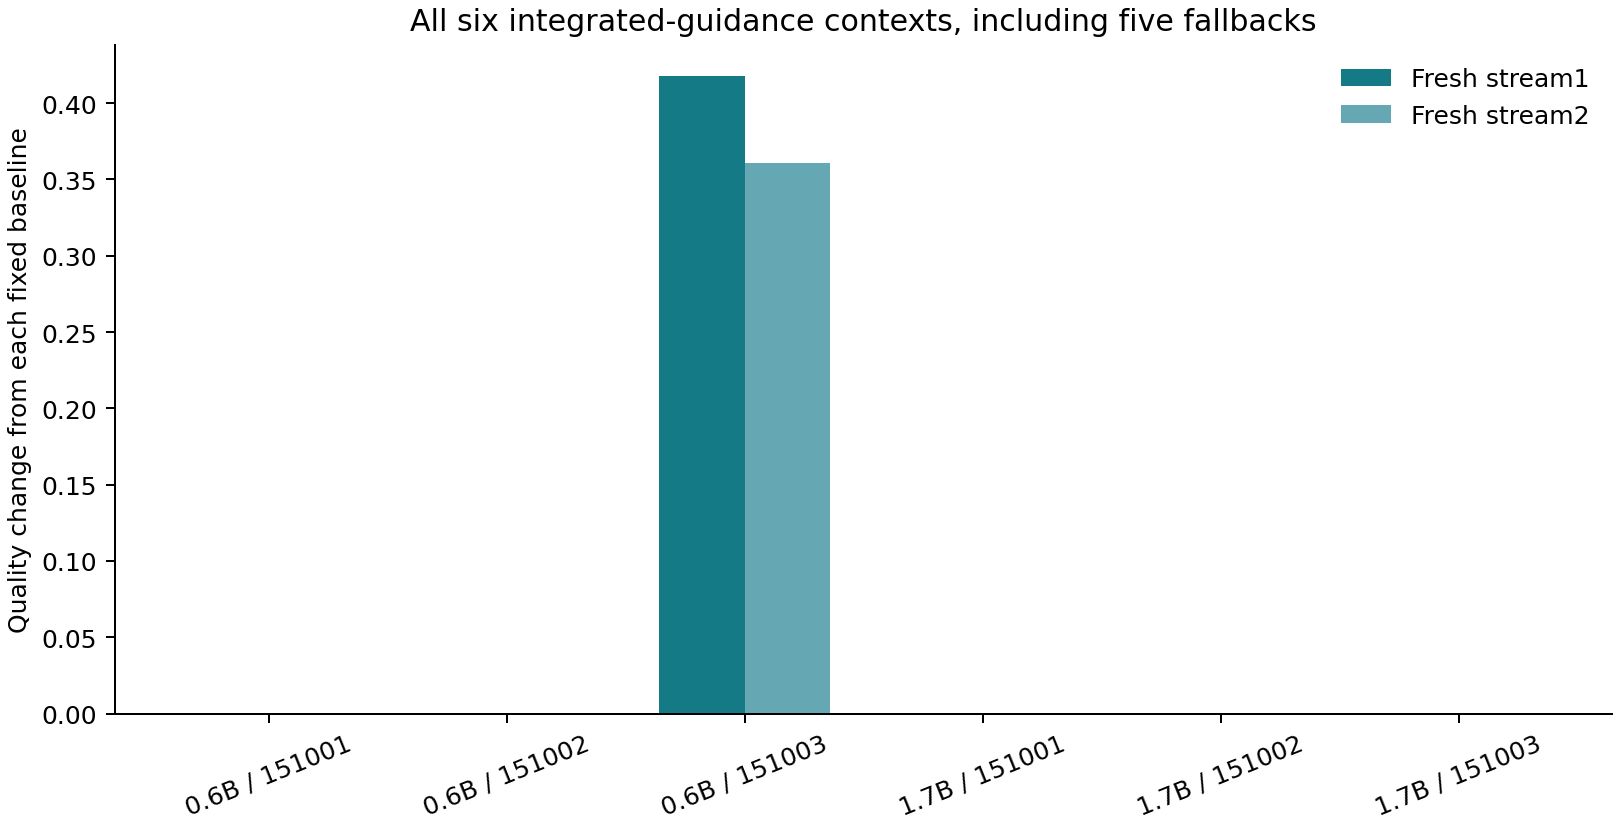
\includegraphics[width=\linewidth]{all-integrated-contexts.png}
\caption{All integrated-guidance contexts. Five retain their baseline. The improvement in the remaining context stays in both fresh streams.}\label{fig:all}
\end{figure}

\section{Resource ledger and independent verification}
The numerical experiment takes 41.32 seconds in the recorded single-thread-configured CPU environment, with whole-process peak RSS 94.23 MiB. This excludes preparation in a separate process. It evaluates 6,928,320 selected fragment responses, 69,120 additional source/diagnostic component responses and 2,280,960 scalar partials. The controller evaluates 36,387,504 component-interface predictions and 41,569,920 routing comparisons. These are distinct work counters; no component count is presented as hardware FLOPs or electrical energy.

Conservative saved pretrained runtime arrays occupy 994,912 bytes for each 0.6B-derived context and 1,740,384 bytes for each 1.7B-derived context, including component rows, coordinate contractions and response interfaces. A selected return uses 1,536 bytes; a shared observation interface and normalizations use 5,376 bytes. Readout libraries and all unsuccessful source/candidate trials are recorded separately. Random-control arrays use larger stored floating-point representations, so storage is reported per arm rather than declared matched.

Preparation is material work. Each extraction executes 294 original gate projections, 294 up projections and 72 down projections, with 294 normalizations, and materializes 2,312,110,080 full-matrix coefficients before retaining the small banks. Those are extraction operations, not a deployed-memory requirement. The original extraction timer captured only the last model; complete initial preparation duration and preparation peak RSS were not recorded. An independent complete extraction takes 2.59 seconds and repeats the same work, yielding identical banks. We include both preparations in the operation ledger and do not infer full-pipeline time, memory or energy savings from the numerical-runtime measurement. Pretraining is inherited, not free work.

Independent replay reconstructs every source readout, shared interface and retained choice, checks 360 seals, and reproduces 1,440 score vectors with maximum absolute $R^2$ difference $3.50\times10^{-10}$. It executes 4,800 saved fields in the original full activation coordinates and reproduces all 9,600 recorded stage-binding choices. Maximum native-output relative discrepancy is $1.20\times10^{-6}$; the maximum absolute discrepancy is $6.49\times10^{-5}$ on larger outputs. These satisfy the inherited native-decomposition tolerance $\mathrm{rtol}=\mathrm{atol}=2\times10^{-5}$. The quadratic integral identity has maximum scaled discrepancy $4.38\times10^{-14}$. This coordinate replay is distinct from the larger mixed-precision extraction discrepancy reported earlier.

The ledger explicitly records verification, independent extraction and partial checking. Two verification-debug attempts used inappropriate absolute-only tolerances before scale-aware native decomposition checks; their extra CPU durations were not captured. Numeric observations, scientific settings and selected constructions were unchanged. We make no net cost saving or measured electricity claim.

\section{Relation to existing building blocks}
Temporal capacity assays measure dynamical information processing~\cite{dambre}. Frozen pretrained transformers have been reused for non-language modalities~\cite{lu}; learned stitching connects fixed representations~\cite{stitch}. These motivate separating pretrained computations from one conventional input/output use. Our earlier component studies supply effect interfaces and native composition~\cite{sg1,sg2}, while the preceding whole-body checkpoint supplies experiential execution/interface selection~\cite{sg4}.

Here the contribution is their executable connection: acquired response/partial interfaces guide a layerless pretrained-fragment runtime, and that runtime completes an acquisition, shared-compatibility, retention and fresh-reuse cycle without the source transformer graph. Quadratic/Hermite fitting, integrated derivatives, magnitude ranking, ridge alignment and finite feedback selection are established numerical tools. The study isolates a concrete construction and its outcomes rather than assigning those tools new priority claims.

\section{The next acquisition}
The retained component construction is a starting state for a second acquisition. A useful next test changes the runtime again while preserving the programs and quality acquired in the first cycle. Some current geometries have no useful measured response complement within their active fragment span. Expanding which physical ports can be recruited, guided by unmet requirements, is therefore a specific developmental target. Future experiments can measure repeated acquisition, composed compatibility, retained-state limits and lifecycle break-even on application tasks. The present result supplies the component-level execution and learning cycle on which that program can operate.

\clearpage
\appendix
\section{Every model, context and control}\label{app:cases}
\begin{table}[ht]\centering\scriptsize\begin{tabular}{lllrrrr}
\toprule
Model & Seed & Guidance & Slot & $\Delta Q_1$ & $\Delta Q_2$ & Old \\
\midrule
0.6B & 151001 & Integrated & 0 & +0.00000 & +0.00000 & 2/2 \\
0.6B & 151001 & First-order & 2 & +0.04269 & +0.03573 & 2/2 \\
0.6B & 151001 & Shuffled & 0 & +0.00000 & +0.00000 & 3/3 \\
0.6B & 151001 & Random weights & 0 & +0.00000 & +0.00000 & 0/0 \\
0.6B & 151002 & Integrated & 0 & +0.00000 & +0.00000 & 5/5 \\
0.6B & 151002 & First-order & 0 & +0.00000 & +0.00000 & 5/5 \\
0.6B & 151002 & Shuffled & 0 & +0.00000 & +0.00000 & 3/3 \\
0.6B & 151002 & Random weights & 0 & +0.00000 & +0.00000 & 5/5 \\
0.6B & 151003 & Integrated & 4 & +0.41753 & +0.36104 & 2/2 \\
0.6B & 151003 & First-order & 1 & +0.42700 & +0.49165 & 1/1 \\
0.6B & 151003 & Shuffled & 4 & +0.04748 & +0.13463 & 1/1 \\
0.6B & 151003 & Random weights & 0 & +0.00000 & +0.00000 & 0/0 \\
1.7B & 151001 & Integrated & 0 & +0.00000 & +0.00000 & 1/1 \\
1.7B & 151001 & First-order & 0 & +0.00000 & +0.00000 & 2/2 \\
1.7B & 151001 & Shuffled & 2 & +0.05250 & -0.04831 & 2/2 \\
1.7B & 151001 & Random weights & 3 & +0.14383 & +0.09988 & 4/4 \\
1.7B & 151002 & Integrated & 0 & +0.00000 & +0.00000 & 3/3 \\
1.7B & 151002 & First-order & 0 & +0.00000 & +0.00000 & 4/4 \\
1.7B & 151002 & Shuffled & 0 & +0.00000 & +0.00000 & 1/1 \\
1.7B & 151002 & Random weights & 0 & +0.00000 & +0.00000 & 0/0 \\
1.7B & 151003 & Integrated & 0 & +0.00000 & +0.00000 & 5/5 \\
1.7B & 151003 & First-order & 0 & +0.00000 & +0.00000 & 5/5 \\
1.7B & 151003 & Shuffled & 0 & +0.00000 & +0.00000 & 4/4 \\
1.7B & 151003 & Random weights & 0 & +0.00000 & +0.00000 & 6/6 \\
\bottomrule
\end{tabular}

\caption{All 24 locked choices. $\Delta Q$ gives absolute fresh-score changes. Old counts use the fixed eligible program set. Zero-action fallbacks are included.}\label{tab:cases}
\end{table}

\section{Reproduction and artifact boundary}
The companion contains the complete captured study, all 24 runtime contexts and five candidate returns, source/development/fresh trajectories, unchanged programs, acquired interfaces, bank provenance, independent replay and generated reports. CPU reproduction needs NumPy; reporting additionally uses Matplotlib. Replay needs no original checkpoint or hosted service. Optional guarded extraction verification uses the pinned MLX checkpoints and records precision tolerances. Full source models are downloaded separately. Extracted/derived arrays retain the upstream model attribution.

The source revisions are:
\begin{quote}\small
0.6B: \texttt{173234aa840d113125e9f2271100ddbaf16c9620}\\
1.7B: \texttt{21457c6f51ed54a7c16e988c0844db973815c137}
\end{quote}
Original component data and experiment outcomes are preserved. Portable wrappers change path handling and add reproducible CLI entry points; those transformations are recorded. Original local source snapshots and their hashes identify the executed experiment. No arXiv identifier has been assigned.

\clearpage
\begin{thebibliography}{9}\small\setlength{\itemsep}{2pt}\raggedright
\bibitem{sg1} N. Oh and P. Attie. Shaping Gap Benchmark: Effect Interfaces for Compositional Execution of Frozen Neural Computation. Repository paper, 2026. \url{https://github.com/calysteon/shaping-gap-benchmark/blob/main/paper/shaping-gap-benchmark.pdf}.
\bibitem{sg2} N. Oh and P. Attie. Shaping Gap Benchmark II: Scalable Effect-Interface Evaluation and Verified Functional Construction. Repository paper, 2026. \url{https://github.com/calysteon/shaping-gap-benchmark/tree/main/checkpoints/02-scaling-and-functions}.
\bibitem{sg4} N. Oh and P. Attie. Shaping Gap Benchmark IV: Experience-Acquired Execution and Compatibility Reuse. Repository paper, 2026. \url{https://github.com/calysteon/shaping-gap-benchmark/tree/main/checkpoints/04-experience-acquired-reuse}.
\bibitem{dambre} J. Dambre, D. Verstraeten, B. Schrauwen and S. Massar. Information Processing Capacity of Dynamical Systems. \emph{Scientific Reports} 2, 514, 2012. \url{https://doi.org/10.1038/srep00514}.
\bibitem{lu} K. Lu, A. Grover, P. Abbeel and I. Mordatch. Pretrained Transformers as Universal Computation Engines. 2021. \url{https://arxiv.org/abs/2103.05247}.
\bibitem{stitch} Y. Bansal, P. Nakkiran and B. Barak. Revisiting Model Stitching to Compare Neural Representations. \emph{NeurIPS}, 2021. \url{https://arxiv.org/abs/2106.07682}.
\end{thebibliography}
\end{document}
